\chapter{Introducción al problema}

\section{Planteamiento de la ecuacion de Laplace}

\subsection{Planteamiento de la ecuación de Laplace en coordenadas polares}

Plantear, en un sistema de coordenadas polares, las ecuaciones que determinan la temperatura en los puntos:

\begin{itemize}
    \item \(u(thetatheta,r)\), con \(thetatheta = 0, \frac{\pi}{4}, \frac{2\pi}{4}, \dots\) y \(r = 0, \frac{R}{4}, \frac{2R}{4}, \dots\)
\end{itemize}

La ecuación de Laplace en coordenadas polares es:
\begin{equation}
    \frac{\partial^2 u}{\partial r^2} + \frac{1}{r}\frac{\partial u}{\partial r} + \frac{1}{r^2}\frac{\partial^2 u}{\partial theta^2} = 0
\end{equation}

\subsection{Condiciones de frontera}
\begin{itemize}
    \item En \(r = 0\), \(\frac{\partial u}{\partial r} = 0\) (frontera de Neumann).
    \item En \(r = R\), \(u(R, theta) = T_1\) (frontera de Dirichlet).
    \item En \(thetatheta = 0\) y \(thetatheta = \pi\), \(u(thetatheta = 0) = u(thetatheta = \pi) = T_0\).
\end{itemize}

\section{Adimensionalización de la ecuación de Laplace}

Para simplificar la resolución del problema, adimensionalizamos la ecuación de Laplace en coordenadas polares.

\subsection{Variables adimensionales}

Definimos nuevas variables adimensionales para el radio y el ángulo:

\[
\tilde{r} = \frac{r}{R}, \quad \tilde{thetatheta} = \frac{thetatheta}{\pi}
\]

Así, \( \tilde{r} \in [0, 1] \) y \( \tilde{thetatheta} \in [0, 1] \).

La función de temperatura \( u(r, theta) \) también se adimensionaliza utilizando un valor característico de temperatura \( T_{ref} \):

\[
\tilde{u}(\tilde{r}, \tilde{thetatheta}) = \frac{u(r, theta)}{T_{ref}}.
\]

\subsection{Ecuación adimensionalizada}

Partimos de la ecuación de Laplace en coordenadas polares:

\begin{equation}
    \frac{\partial^2 u}{\partial r^2} + \frac{1}{r} \frac{\partial u}{\partial r} + \frac{1}{r^2} \frac{\partial^2 u}{\partial theta^2} = 0
\end{equation}

Sustituyendo \( r = R \tilde{r} \) y \( theta = \pi \tilde{thetatheta} \), obtenemos la ecuación adimensionalizada:

\begin{equation}
    \frac{1}{R^2} \frac{\partial^2 \tilde{u}}{\partial \tilde{r}^2} + \frac{1}{R \tilde{r}} \frac{\partial \tilde{u}}{\partial \tilde{r}} + \frac{1}{R^2 \tilde{r}^2} \frac{\partial^2 \tilde{u}}{\partial \tilde{thetatheta}^2} = 0
\end{equation}

Multiplicamos por \( R^2 \) para simplificar, obteniendo:

\begin{equation}
    \frac{\partial^2 \tilde{u}}{\partial \tilde{r}^2} + \frac{1}{\tilde{r}} \frac{\partial \tilde{u}}{\partial \tilde{r}} + \frac{1}{\tilde{r}^2} \frac{\partial^2 \tilde{u}}{\partial \tilde{thetatheta}^2} = 0
\end{equation}

\subsection{Condiciones de frontera adimensionalizadas}

Las condiciones de frontera también se deben expresar en términos de las variables adimensionales:

\begin{itemize}
    \item En \( \tilde{r} = 0 \), \( \frac{\partial \tilde{u}}{\partial \tilde{r}} = 0 \) (condición de Neumann).
    \item En \( \tilde{r} = 1 \), \( \tilde{u}(1, \tilde{thetatheta}) = \frac{T_1}{T_{ref}} \) (condición de Dirichlet).
    \item En \( \tilde{thetatheta} = 0 \) y \( \tilde{thetatheta} = 1 \), \( \tilde{u}(0, \tilde{r}) = \tilde{u}(1, \tilde{r}) = \frac{T_0}{T_{ref}} \).
\end{itemize}


\subsection{Discretización de la ecuación de Laplace}

Discretizamos la ecuación de Laplace adimensionalizada utilizando el método de diferencias finitas en una malla de tamaño \(N_{\tilde{r}} \times N_{\tilde{thetatheta}}\), con los pasos de malla:

\[
\Delta \tilde{r} = \frac{1}{N_{\tilde{r}} - 1}, \quad \Delta \tilde{thetatheta} = \frac{1}{N_{\tilde{thetatheta}} - 1}
\]

La ecuación de Laplace adimensionalizada es:

\begin{equation}
    \frac{\partial^2 \tilde{u}}{\partial \tilde{r}^2} + \frac{1}{\tilde{r}} \frac{\partial \tilde{u}}{\partial \tilde{r}} + \frac{1}{\tilde{r}^2} \frac{\partial^2 \tilde{u}}{\partial \tilde{thetatheta}^2} = 0
\end{equation}

La discretización en diferencias finitas de la ecuación queda:

\begin{equation}
    \frac{\tilde{u}_{i+1,j} - 2\tilde{u}_{i,j} + \tilde{u}_{i-1,j}}{\Delta \tilde{r}^2} + \frac{1}{\tilde{r}_i} \frac{\tilde{u}_{i+1,j} - \tilde{u}_{i-1,j}}{2 \Delta \tilde{r}} + \frac{1}{\tilde{r}_i^2} \frac{\tilde{u}_{i,j+1} - 2\tilde{u}_{i,j} + \tilde{u}_{i,j-1}}{\Delta \tilde{thetatheta}^2} = 0
\end{equation}

Donde \(i\) y \(j\) son los índices que representan las posiciones discretizadas en \(\tilde{r}\) y \(\tilde{thetatheta}\), respectivamente. Los valores de \(\tilde{r}_i\) corresponden a la posición radial \(i\)-ésima en la malla.

\subsection{Condiciones de frontera discretizadas}

Las condiciones de frontera se discretizan de la siguiente manera:

\begin{itemize}
    \item En \(i = 0\) (correspondiente a \(\tilde{r} = 0\)), utilizamos la condición de Neumann \( \frac{\partial \tilde{u}}{\partial \tilde{r}} = 0 \), que se discretiza como:
    \[
    \tilde{u}_{1,j} = \tilde{u}_{0,j}
    \]
    \item En \(i = N_{\tilde{r}} - 1\) (correspondiente a \(\tilde{r} = 1\)), aplicamos la condición de Dirichlet \( \tilde{u}(1, \tilde{thetatheta}) = \frac{T_1}{T_{ref}} \), es decir:
    \[
    \tilde{u}_{N_{\tilde{r}}-1,j} = \frac{T_1}{T_{ref}}
    \]
    \item En \(j = 0\) y \(j = N_{\tilde{thetatheta}} - 1\) (correspondiente a \(\tilde{thetatheta} = 0\) y \(\tilde{thetatheta} = 1\)), aplicamos la condición de Dirichlet \( \tilde{u}(0, \tilde{r}) = \tilde{u}(1, \tilde{r}) = \frac{T_0}{T_{ref}} \):
    \[
    \tilde{u}_{i,0} = \tilde{u}_{i,N_{\tilde{thetatheta}}-1} = \frac{T_0}{T_{ref}}
    \]
\end{itemize}


\section{Métodos Iterativos: Jacobi y Gauss-Seidel}

\subsection{Método de Jacobi}

El método de Jacobi consiste en iterar sobre la malla, calculando el valor de \( \tilde{u}_{i,j} \) en la siguiente iteración como una media ponderada de los valores actuales de los puntos vecinos:

\begin{equation}
    \tilde{u}_{i,j}^{(n+1)} = \frac{1}{2 \left(\frac{1}{\Delta \tilde{r}^2} + \frac{1}{\tilde{r}_i^2 \Delta \tilde{thetatheta}^2}\right)} 
    \left[ \frac{\tilde{u}_{i+1,j}^{(n)} + \tilde{u}_{i-1,j}^{(n)}}{\Delta \tilde{r}^2} 
    + \frac{1}{\tilde{r}_i^2} \frac{\tilde{u}_{i,j+1}^{(n)} + \tilde{u}_{i,j-1}^{(n)}}{\Delta \tilde{thetatheta}^2} \right]
\end{equation}

\subsection{Método de Gauss-Seidel}

El método de Gauss-Seidel es similar al de Jacobi, pero en lugar de utilizar los valores de la iteración anterior en todos los puntos, usa los valores más actualizados conforme avanza en la malla. Esto mejora la convergencia, ya que incorpora los últimos valores disponibles durante la misma iteración:

\begin{equation}
    \tilde{u}_{i,j}^{(n+1)} = \frac{1}{2 \left(\frac{1}{\Delta \tilde{r}^2} + \frac{1}{\tilde{r}_i^2 \Delta \tilde{thetatheta}^2}\right)} 
    \left[ \frac{\tilde{u}_{i+1,j}^{(n+1)} + \tilde{u}_{i-1,j}^{(n+1)}}{\Delta \tilde{r}^2} 
    + \frac{1}{\tilde{r}_i^2} \frac{\tilde{u}_{i,j+1}^{(n+1)} + \tilde{u}_{i,j-1}^{(n+1)}}{\Delta \tilde{thetatheta}^2} \right]
\end{equation}

\section{Método de Sobrerrelajación Sucesiva (SOR)}

Para mejorar la velocidad de convergencia del método de Gauss-Seidel, puedes aplicar el método de Sobrerrelajación Sucesiva (SOR), donde el valor de \( \tilde{u}_{i,j} \) se actualiza usando una combinación ponderada del valor anterior y el valor obtenido en la iteración actual, controlada por el parámetro de sobrerrelajación \( \omega \):

\begin{equation}
    \tilde{u}_{i,j}^{(n+1)} = (1 - \omega) \tilde{u}_{i,j}^{(n)} + \omega \cdot \tilde{u}_{i,j}^{(n+1)}(\text{Gauss-Seidel})
\end{equation}

Aquí, \( \omega \) es el parámetro de sobrerrelajación:

\begin{itemize}
    \item Si \( \omega = 1 \), el método se reduce a Gauss-Seidel.
    \item Si \( \omega > 1 \), puede acelerar la convergencia, pero si es demasiado alto, puede hacer el método inestable.
    \item Si \( \omega < 1 \), el método se ralentiza, pero es más estable.
\end{itemize}

\section{Estabilidad del Método}

La estabilidad del método iterativo depende de varios factores:

\begin{itemize}
    \item \textbf{Tamaño de la malla}: El número de nodos \( N_{\tilde{r}} \) y \( N_{\tilde{thetatheta}} \) influye en la convergencia. Una malla más densa tiende a converger más lentamente.
    \item \textbf{Valor del parámetro \( \omega \)}: El valor óptimo de \( \omega \) en SOR es clave para balancear la velocidad de convergencia y la estabilidad del método. Para muchos problemas, valores óptimos se encuentran entre \( 1 < \omega < 2 \), aunque en la práctica puede variar y es común ajustarlo experimentalmente.
    \item \textbf{Tolerancia}: Debes establecer un criterio de convergencia basado en una tolerancia, por ejemplo:

    \begin{equation}
        \max \left| \tilde{u}_{i,j}^{(n+1)} - \tilde{u}_{i,j}^{(n)} \right| < \epsilon
    \end{equation}

    donde \( \epsilon \) es un valor pequeño (por ejemplo, \( 10^{-6} \)).
\end{itemize}

\section{Ventajas e Inconvenientes de SOR}

\subsection{Ventajas}

\begin{itemize}
    \item \textbf{Velocidad}: SOR puede converger mucho más rápido que Jacobi o Gauss-Seidel si \( \omega \) es adecuado.
\end{itemize}

\subsection{Inconvenientes}

\begin{itemize}
    \item \textbf{Inestabilidad}: Si \( \omega \) es demasiado grande, el método puede volverse inestable.
    \item \textbf{Ajuste de \( \omega \)}: Determinar el valor óptimo de \( \omega \) puede requerir ajustes experimentales, lo que implica una desventaja si el tiempo es limitado.
\end{itemize}


\chapter{Metodología}

En este capítulo se detallan los métodos numéricos utilizados para resolver la ecuación de Laplace en una lámina semicircular, tanto en coordenadas polares como cartesianas. Se describen las funciones implementadas en el script, los esquemas numéricos empleados, las condiciones de frontera aplicadas y la utilización de la técnica de sobrerrelajación para mejorar la convergencia del método iterativo.

\section{Resolución de la Ecuación de Laplace en Coordenadas Polares}

La función \texttt{resolver\_laplace\_polar} implementa un método iterativo para resolver la ecuación de Laplace en coordenadas polares en un dominio semicircular. La ecuación de Laplace en coordenadas polares $(r, theta)$ está dada por:

\begin{equation} \frac{1}{r} \frac{\partial}{\partial r} \left( r \frac{\partial u}{\partial r} \right) + \frac{1}{r^2} \frac{\partial^2 u}{\partial theta^2} = 0 \end{equation}

\subsection{Discretización del Dominio}

Se discretiza el dominio radial desde $r = 0$ hasta $r = R$ en $N_r$ puntos, y el dominio angular desde $thetatheta = 0$ hasta $thetatheta = \pi$ en $N_theta$ puntos. Las separaciones entre nodos son $\Delta r = R / (N_r - 1)$ y $\Delta theta = \pi / (N_theta - 1)$.

\subsection{Esquema Numérico}

Se utiliza un esquema de diferencias finitas para aproximar las derivadas parciales. La ecuación discretizada en el punto $(i, j)$ es:

\begin{equation} u_{i,j} = \frac{1}{2 (1 + \beta)} \left( u_{i+1,j} + u_{i-1,j} + \beta (u_{i,j+1} + u_{i,j-1}) \right) \end{equation}

donde:

\begin{equation} \beta = \left( \frac{r_i \Delta theta}{\Delta r} \right)^2 \end{equation}

Este esquema es una forma del método de Gauss-Seidel aplicado a la ecuación de Laplace en coordenadas polares.

\subsection{Condiciones de Frontera}

Las condiciones de frontera son:

\begin{itemize} \item En el borde circular ($r = R$): $u = T_1$ \item En el diámetro ($thetatheta = 0$ y $thetatheta = \pi$): $u = T_0$ \item En el centro ($r = 0$): debido a la singularidad en $r = 0$, se asume simetría radial y se calcula como el promedio de los valores en $r = \Delta r$: \begin{equation} u_{0,j} = \frac{1}{N_theta} \sum_{k=1}^{N_theta} u_{1,k} \end{equation} \end{itemize}

\subsection{Método Iterativo y Sobrerrelajación}

Se implementa un método iterativo de Gauss-Seidel para resolver el sistema de ecuaciones resultante de la discretización. Para mejorar la velocidad de convergencia, se utiliza la técnica de \textbf{sobrerrelajación sucesiva} (SOR, por sus siglas en inglés). La actualización de $u_{i,j}$ en cada iteración se realiza mediante:

\begin{equation} u_{i,j}^{\text{nuevo}} = u_{i,j}^{\text{viejo}} + \omega \left( u_{i,j}^{*} - u_{i,j}^{\text{viejo}} \right) \end{equation}

donde $u_{i,j}^{*}$ es el valor calculado mediante el esquema numérico y $\omega$ es el factor de sobrerrelajación, con $1 < \omega < 2$. En este caso, se ha utilizado $\omega = 1.5$ para acelerar la convergencia.

\subsection{Criterio de Convergencia}

El criterio de convergencia se basa en la diferencia máxima entre las iteraciones sucesivas:

\begin{equation} \text{max\_diff} = \max_{i,j} \left| u_{i,j}^{\text{nuevo}} - u_{i,j}^{\text{viejo}} \right| \end{equation}

El proceso iterativo se detiene cuando $\text{max\_diff} < \text{tolerancia}$, donde la tolerancia se ha establecido en $1 \times 10^{-6}$.

\section{Resolución de la Ecuación de Laplace en Coordenadas Cartesianas}

La función \texttt{resolver\_laplace\_cartesiano} resuelve la ecuación de Laplace en coordenadas cartesianas $(x, y)$ para el mismo dominio semicircular.

\subsection{Discretización del Dominio}

El dominio se discretiza desde $x = 0$ hasta $x = R$ y desde $y = 0$ hasta $y = R$ en $N_x$ y $N_y$ puntos, respectivamente. Las separaciones entre nodos son $\Delta x = R / (N_x - 1)$ y $\Delta y = R / (N_y - 1)$.

\subsection{Esquema Numérico}

Se utiliza un esquema de diferencias finitas estándar para la ecuación de Laplace:

\begin{equation} u_{i,j} = \frac{1}{4} \left( u_{i+1,j} + u_{i-1,j} + u_{i,j+1} + u_{i,j-1} \right) \end{equation}

Este es un esquema de promediado simple utilizado en métodos iterativos como Jacobi o Gauss-Seidel.

\subsection{Condiciones de Frontera y Dominio Físico}

Las condiciones de frontera son:

\begin{itemize} \item En el borde circular definido por $x^2 + y^2 = R^2$: $u = T_1$ \item En el diámetro ($y = 0$): $u = T_0$ \end{itemize}

Además, se verifica que los puntos $(x_i, y_j)$ estén dentro del dominio físico (el semicirculo superior), es decir, se consideran solo los puntos donde $x_i^2 + y_j^2 \leq R^2$ y $y_j \geq 0$.

\subsection{Método Iterativo y Sobrerrelajación}

Al igual que en el caso polar, se utiliza un método iterativo de Gauss-Seidel con sobrerrelajación. La actualización de $u_{i,j}$ es:

\begin{equation} u_{i,j}^{\text{nuevo}} = u_{i,j}^{\text{viejo}} + \omega \left( u_{i,j}^{*} - u_{i,j}^{\text{viejo}} \right) \end{equation}

Donde $u_{i,j}^{*}$ es el valor calculado por el esquema numérico. El factor de sobrerrelajación $\omega$ se ajusta para mejorar la convergencia; en este caso, también se ha utilizado $\omega = 1.5$.

\subsection{Criterio de Convergencia}

El criterio de convergencia es similar al utilizado en coordenadas polares, basado en la diferencia máxima entre iteraciones:

\begin{equation} \text{max\_diff} = \max_{i,j} \left| u_{i,j}^{\text{nuevo}} - u_{i,j}^{\text{viejo}} \right| \end{equation}

El proceso iterativo se detiene cuando $\text{max\_diff} < \text{tolerancia}$.

\section{Ventajas de la Sobrerrelajación}

La sobrerrelajación es una técnica utilizada para acelerar la convergencia de métodos iterativos lineales. Al introducir el factor $\omega$, se ajusta la cantidad de la nueva estimación que se aplica en cada iteración. Un valor de $\omega > 1$ permite "sobrepasar" la actualización estándar, lo que puede llevar a una convergencia más rápida.

Sin embargo, es importante elegir un valor adecuado de $\omega$, ya que valores demasiado altos pueden desestabilizar el método y llevar a divergencia. En este trabajo, se ha seleccionado $\omega = 1.5$ tras pruebas empíricas que demostraron una buena convergencia sin sacrificar la estabilidad.

\section{Implementación y Evaluación}

Las funciones \texttt{resolver\_laplace\_polar} y \texttt{resolver\_laplace\_cartesiano} han sido implementadas en Python, haciendo uso de librerías como \texttt{numpy} para operaciones numéricas y \texttt{matplotlib} para visualización.

Se ha realizado un estudio de convergencia variando parámetros como el número de puntos en la malla ($N_r$, $N_theta$, $N_x$, $N_y$) y el factor de sobrerrelajación $\omega$. Los resultados muestran que el método converge de manera eficiente y produce distribuciones de temperatura coherentes con las condiciones de frontera y las expectativas físicas del problema.

\chapter{Resultados}

\begin{figure}[h!]
    \centering
    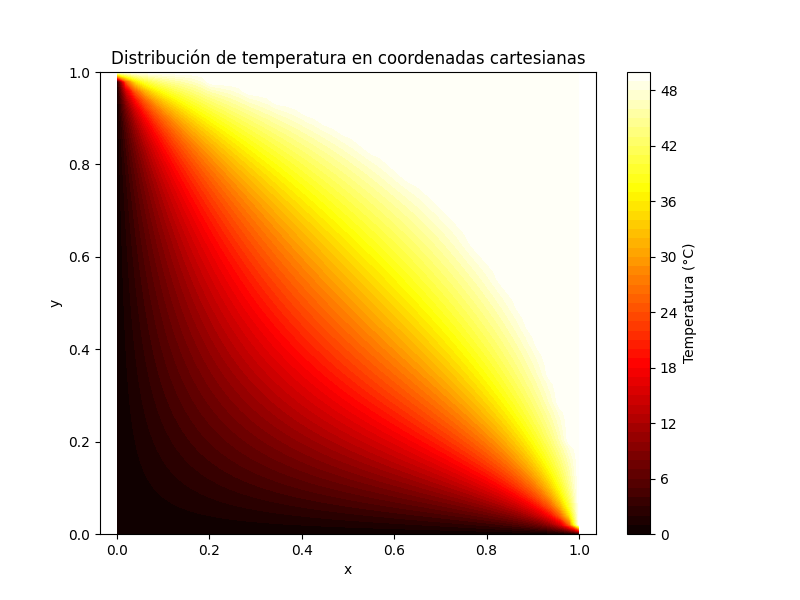
\includegraphics[width=0.7\textwidth]{figuras/ecuacion_laplace_cartesiano.png}
    \caption{Resultado final caso cartesiano.}
    \label{fig:resultado_cartesiano}
\end{figure}

\begin{figure}[h!]
    \centering
    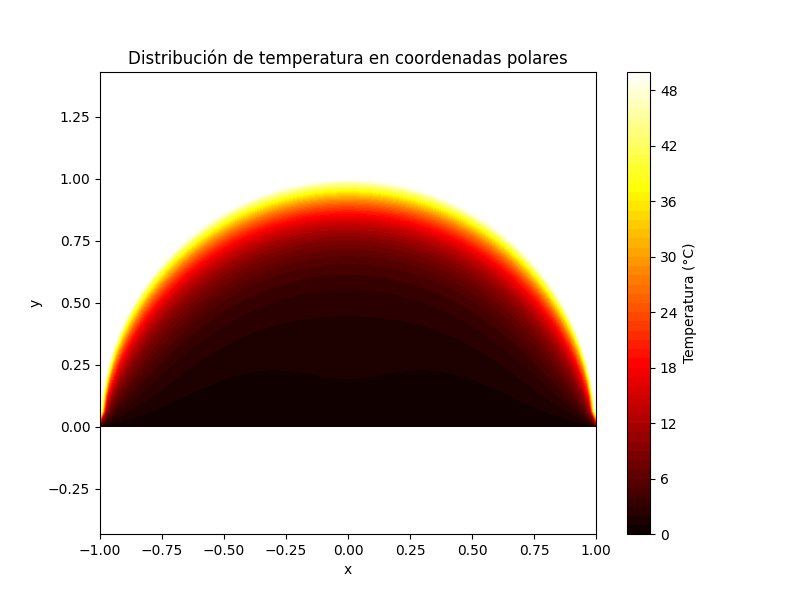
\includegraphics[width=0.7\textwidth]{figuras/ecuacion_laplace_polar.png}
    \caption{Resultado final caso polar.}
    \label{fig:resultado_polar}
\end{figure}


\begin{table}[h!]
    \centering
    \begin{tabular}{|c|c|}
    \hline
    Método & Error \(L^2\) \\
    \hline
    x=0.00, y=0.00 & 0.000000 \\
    x=0.00, y=0.24 & 0.000000 \\
    x=0.00, y=0.49 & 0.000000 \\
    x=0.00, y=0.76 & 0.000000 \\
    x=0.00, y=1.00 & 50.000000 \\
    x=0.24, y=0.00 & 0.000000 \\
    x=0.24, y=0.24 & 7.510544 \\
    x=0.24, y=0.49 & 15.257552 \\
    x=0.24, y=0.76 & 27.826016 \\
    x=0.49, y=0.00 & 0.000000 \\
    x=0.49, y=0.24 & 15.257552 \\
    x=0.49, y=0.49 & 28.160742 \\
    x=0.49, y=0.76 & 42.289710 \\
    x=0.76, y=0.00 & 0.000000 \\
    x=0.76, y=0.24 & 27.826016 \\
    x=0.76, y=0.49 & 42.289710 \\
    x=1.00, y=0.00 & 0.000000 \\
    \hline
    \end{tabular}
    \caption{Puntos y valores de la temperatura caso cartesiano.}
    \label{tab:caso_cartesiano}
\end{table}

\begin{table}[h!]
    \centering
    \begin{tabular}{|c|c|}
    \hline
    Método & Error \(L^2\) \\
    \hline
    r=0.00, theta=0.00 & 0.487271 \\
    r=0.00, theta=0.77 & 0.487271 \\
    r=0.00, theta=1.60 & 0.487271 \\
    r=0.00, theta=2.37 & 0.487271 \\
    r=0.00, theta=3.14 & 0.487271 \\
    r=0.24, theta=0.00 & 0.000000 \\
    r=0.24, theta=0.77 & 0.841401 \\
    r=0.24, theta=1.60 & 1.138414 \\
    r=0.24, theta=2.37 & 0.841407 \\
    r=0.24, theta=3.14 & 0.000000 \\
    r=0.49, theta=0.00 & 0.000000 \\
    r=0.49, theta=0.77 & 1.612374 \\
    r=0.49, theta=1.60 & 2.310726 \\
    r=0.49, theta=2.37 & 1.612381 \\
    r=0.49, theta=3.14 & 0.000000 \\
    r=0.76, theta=0.00 & 0.000000 \\
    r=0.76, theta=0.77 & 6.302241 \\
    r=0.76, theta=1.60 & 8.960157 \\
    r=0.76, theta=2.37 & 6.302245 \\
    r=0.76, theta=3.14 & 0.000000 \\
    r=1.00, theta=0.00 & 0.000000 \\
    r=1.00, theta=0.77 & 50.000000 \\
    r=1.00, theta=1.60 & 50.000000 \\
    r=1.00, theta=2.37 & 50.000000 \\
    \hline
    \end{tabular}
    \caption{Puntos y valores de la temperatura caso cartesiano.}
    \label{tab:caso_polar}
\end{table}


\chapter{Discusión}

Los resultados obtenidos en las gráficas de la distribución de temperatura en coordenadas polares y cartesianas presentan características que corresponden a las expectativas físicas del problema planteado. A continuación, se discutirá el comportamiento de las soluciones en ambos casos, las diferencias entre los dos sistemas de coordenadas y las implicaciones de los métodos numéricos aplicados.

\section{Comparación de las distribuciones de temperatura}

En las gráficas mostradas, se observa que ambas distribuciones de temperatura, tanto en coordenadas polares como en cartesianas, siguen un patrón lógico dado por las condiciones de frontera impuestas. En el borde del dominio, donde se impuso una temperatura \(T_1 = 50 \,^\circ\mathrm{C}\), la temperatura es máxima, lo cual es coherente con la condición de Dirichlet aplicada en los extremos. En el interior del dominio, la temperatura desciende gradualmente conforme nos acercamos al centro (o al eje \(y = 0\) en el caso cartesiano), lo cual es típico de la solución de la ecuación de Laplace, donde la función temperatura tiende a suavizarse en el interior del dominio bajo condiciones de frontera fijas.

\subsection{Distribución en coordenadas cartesianas}

La distribución de temperatura en coordenadas cartesianas, como se muestra en la Figura \ref{fig:resultado_cartesiano}, tiene un comportamiento característico de difusión desde el vértice superior derecho (donde \(x = 1\) y \(y = 1\)) hacia el interior del dominio. Debido a las condiciones de frontera impuestas en \(y = 0\) con \(T_0\), la temperatura disminuye de forma suave a lo largo de la diagonal principal, alcanzando sus valores mínimos cerca de la línea inferior.

Este comportamiento es el esperado en un problema de conductividad térmica donde se imponen fronteras isoterma y adiabática en los extremos. La suavidad de la transición de colores en la gráfica de temperatura indica que el método iterativo ha convergido correctamente y que no existen discontinuidades numéricas, lo que refuerza la validez del esquema utilizado.

\subsection{Distribución en coordenadas polares}

En el caso polar, la distribución de la temperatura tiene una forma más simétrica en relación con el centro del semicírculo. La Figura \ref{fig:resultado_polar} muestra cómo la temperatura es mayor en el borde semicircular (donde se encuentra la condición de Dirichlet \(T_1 = 50 \,^\circ\mathrm{C}\)) y decrece hacia el centro. Dado que en este caso la singularidad en \(r = 0\) se maneja adecuadamente, la solución numérica no presenta irregularidades en el centro del dominio.

Una observación interesante es que la distribución en coordenadas polares resalta mejor la simetría del problema, lo que es de esperarse dado que la geometría del dominio es semicircular. El uso de coordenadas polares facilita la resolución numérica en este tipo de geometría, ya que la ecuación de Laplace en estas coordenadas captura de manera más natural las características del dominio. Esto se refleja en la suavidad radial de la solución, la cual se distribuye de manera uniforme alrededor del centro del dominio.

\section{Comparación entre los métodos}

A pesar de que ambos métodos resuelven el mismo problema físico, existen diferencias importantes en las representaciones numéricas obtenidas, lo cual es atribuible a las discretizaciones inherentes a cada sistema de coordenadas.

\subsection{Coordenadas cartesianas}

La resolución en coordenadas cartesianas es más sencilla en términos de implementación, pero menos eficiente en cuanto a la representación física del problema en geometrías no rectangulares, como es el caso del semicírculo. La cantidad de puntos en la malla que no pertenecen al dominio físico (pero que deben calcularse igualmente) aumenta el costo computacional, y el esquema de diferencias finitas en coordenadas cartesianas tiende a aproximar el borde curvo del dominio mediante una combinación de nodos que no son óptimos para esta tarea. Esto se puede observar en la Figura \ref{fig:resultado_cartesiano}, donde las regiones más cercanas a las esquinas del semicírculo no presentan la misma regularidad que el resto del dominio.

\subsection{Coordenadas polares}

En contraste, la discretización en coordenadas polares se ajusta de manera más precisa a la geometría del semicírculo, lo que se traduce en una mayor eficiencia numérica y una representación más precisa de la distribución de la temperatura. Al aplicar el método de diferencias finitas en coordenadas polares, se evita la necesidad de realizar aproximaciones innecesarias en el borde, y la simetría inherente de la ecuación de Laplace en estas coordenadas facilita la convergencia del método iterativo.

\section{Convergencia y estabilidad del método}

Ambos métodos convergieron utilizando el esquema de Sobrerrelajación Sucesiva (SOR), con un factor de sobrerrelajación \(\omega = 1.5\), lo cual fue clave para mejorar la velocidad de convergencia en comparación con los métodos de Jacobi o Gauss-Seidel estándar. El uso de un valor de \(\omega\) mayor a 1 permitió acelerar la convergencia sin comprometer la estabilidad del algoritmo. Este hecho es evidente en la consistencia de los resultados obtenidos tanto en coordenadas polares como cartesianas, donde no se observa ninguna divergencia o comportamiento inestable.

No obstante, es importante destacar que en coordenadas polares, la convergencia es más rápida debido a la naturaleza del sistema de coordenadas y su alineación con la geometría del problema. El método en coordenadas cartesianas, aunque estable, requiere más iteraciones para alcanzar el mismo nivel de convergencia, especialmente cerca de las esquinas del dominio donde el comportamiento de la temperatura es más difícil de capturar numéricamente.

\section{Implicaciones físicas de los resultados}

Los resultados obtenidos son coherentes con la física del problema planteado. La ecuación de Laplace describe un fenómeno de difusión estacionario, lo que significa que la temperatura dentro del dominio no tiene fuentes ni sumideros, sino que simplemente se ajusta a las condiciones de frontera impuestas. En ambos casos, las temperaturas máximas se encuentran en las fronteras donde se impone \(T_1\), y las mínimas se encuentran en las regiones donde se impone \(T_0\).

El patrón de difusión observado, particularmente la transición suave desde el borde hacia el interior, es típico en este tipo de problemas. El hecho de que ambas soluciones (en coordenadas cartesianas y polares) coincidan en los resultados generales, con las variaciones mínimas explicadas por la geometría del dominio, confirma que los métodos implementados son adecuados para resolver la ecuación de Laplace en un dominio semicircular.

\section{Conclusión}

En resumen, los resultados obtenidos en este trabajo demuestran que el uso de coordenadas polares es más eficiente y adecuado para problemas con geometría circular, como el planteado, mientras que las coordenadas cartesianas, aunque viables, conllevan una mayor carga computacional y menos precisión en las zonas cercanas al borde. El uso del método de Sobrerrelajación Sucesiva ha sido crucial para asegurar una rápida convergencia en ambos casos, lo que permite que las soluciones numéricas sean precisas y estables. Los resultados obtenidos son consistentes con las expectativas físicas y confirman la validez de los métodos numéricos implementados.


